
\section{実験1}
\subsection{実験の目的,概要}
本実験では,2入力1出力のセレクタ回路を設計し,シュミレーションや論理合成を行って,FPGAボードでの動作を確認する。
これによってHDLによる記述,シュミレータの使い方,回路をFPGA上で動かすための方法を確認する。

入力はD0,D1(1bitデータ),S1(1bitセレクト信号)。
出力はY(1bit)。
セレクタ信号が0ならばD0のデータを,1ならばD1のデータを出力する。

ICE計算機上の,ModelSim,Quartus,FPGAボードはDE10-Liteを使用する。

\subsection{実験方法}
\subsubsection{HDLでの回路記述}
以下のような回路記述をmux.v,テストベンチをtest\_mux.vとして作成する。
\lstinputlisting[caption=mux21.v,label=mux21.v]{./src/mux21/mux21.v}
\lstinputlisting[caption=test\_mux21.v,label=testmux21.v]{./src/mux21/test_mux21.v}

\subsubsection{機能レベルシュミレーション}
作成したテストベンチをもとに,ModelSimで信号波形を出力する。
入出力の値が仕様通りの真理値表と一致することを確認する。

\subsubsection{コンパイル}
以下の2ファイルを作成し,配置する。
\lstinputlisting[caption=mux21.qpf,label=mux21.qpf]{./src/mux21/mux21.qpf}
\lstinputlisting[caption=mux21.qsf,label=mux21.qsf]{./src/mux21/mux21.qsf}

作成した回路記述をQuartusでコンパイルし,論理合成とレイアウトを行う。回路構成やロジックエレメント数,遅延時間について確認する。

\subsubsection{FPGAボードでの回路実現}
計算機にFPGAボードを接続し,dmesgコマンドで接続を確認する。
以下のような設定ファイルを配置し,`quartus-pgm mux21.cdf'を実行して,接続したFPGAにダウンロードする。
\lstinputlisting[caption=mux21.cdf ダウンロード設定ファイル,label=mux21.cdf ダウンロード設定ファイル]{./src/mux21/mux21.cdf}

FPGAが仕様通りに動作するかを確認する。

\subsection{実験結果}
\subsubsection{機能レベルシュミレーション}
ModelSimで波形を作成した結果,以下のような波形になった。

\begin{figure}[H]
  \centering
  
\includegraphics[width=\linewidth]{./src/mux21/mux21_wave11.png}
  \caption{mux21の波形}
\end{figure}

Yの出力値が期待どおりに0→1→0→0で推移し,S1によってD0,D1が切り替わっていることが確認できた。

\subsubsection{論理合成}
論理合成の結果,以下のような回路が作られた。

\begin{figure}[H]
  \centering
  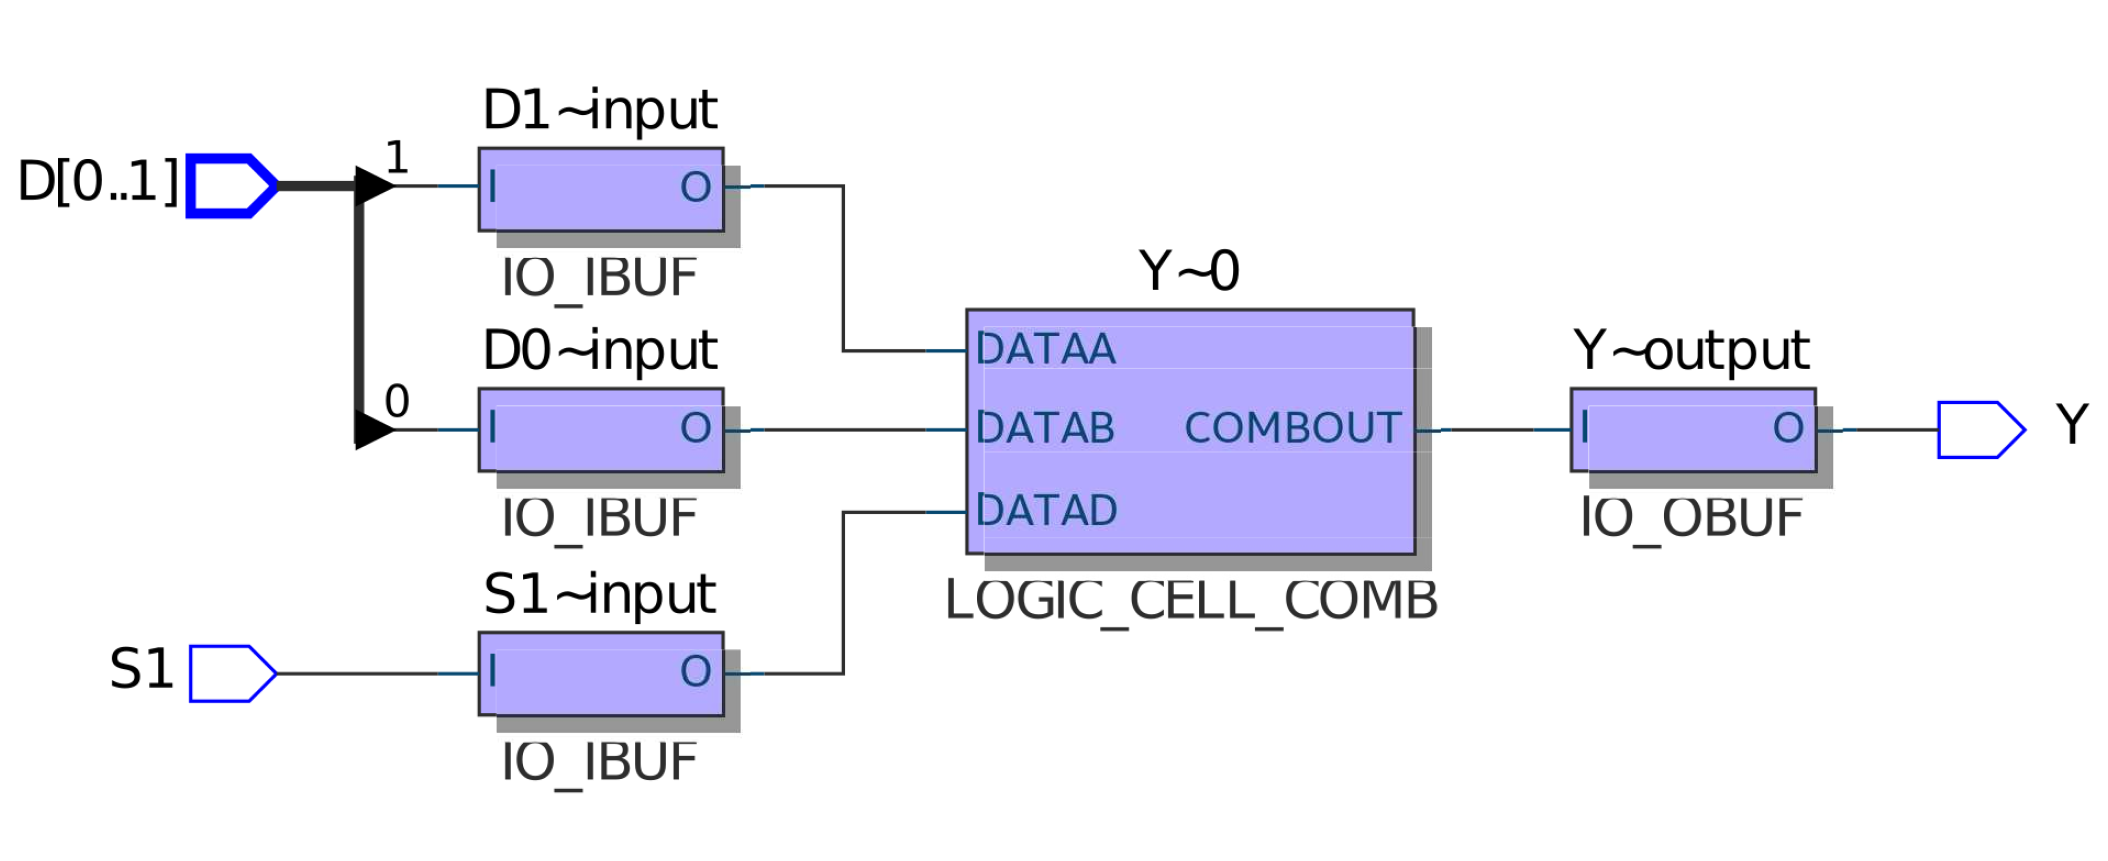
\includegraphics[width=\linewidth]{./src/mux21/mux21_print.png}
  \caption{mux21の回路}
\end{figure}

ロジックエレメント数は2だった。

回路全体の遅延時間は,以下のようになった。
Y~Oの部分で遅延が大きくなった。

\begin{figure}[H]
  \centering
  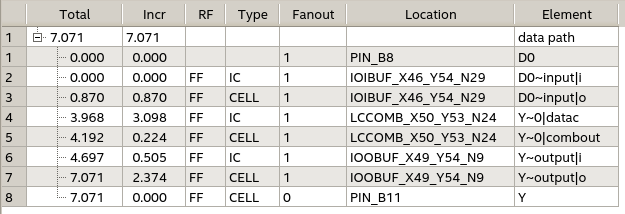
\includegraphics[width=\linewidth]{./src/mux21/mux21Timing.png}
  \caption{mux21の遅延時間}
\end{figure}

\subsubsection{FPGAボードでの動作結果}
スイッチによってS1の値が変わり,それに対応して2つのボタンのうちどちらかの入力がLEDで出力された。
回路記述で割り当てた論理演算通りの入出力だった。

\subsection{考察}
\subsubsection{回路のHDL記述}
コード\ref{mux21.v}では,input output で割り当てた入出力に,assignで単純な論理演算の結果を割り当てている。
Yに$(\lnot{S1} \land D0)|(S1 \land D1)$を割り当てることで,S1の値によってD1とD2のどちらを出力するか選択することができている。
(S1が0の場合D0が,1の場合D1が出力される)

コード\ref{testmux21.v}では,コード\ref{mux21.v}からmux21モジュールを読み込んで動作させながら,20ns間隔で(S1=0, D0=0, D1=0)→(S1=0, D0=1, D1=0)→(S1=1, D0=1, D1=0)→(S1=0, D0=0, D1=0)と入力を遷移させている。

\subsubsection{論理合成}
回路の遅延は,処理が行われているY~Oで大きくなっていた。
実際,以下のようにY~Oにはゲートが配置され,他は入出力用のセルだった。

\begin{figure}[H]
  \centering
  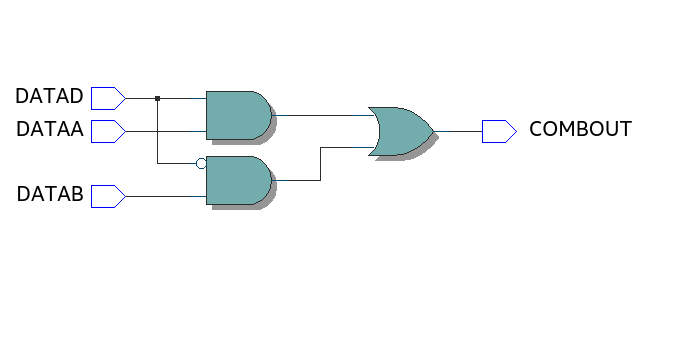
\includegraphics[width=\linewidth]{./src/mux21/mux21elm.png}
  \caption{mux21のゲート}
\end{figure}

また,この結果よりロジックエレメントの値はゲートの数に一致しないことも分かった。\\

この実験で,assign句など,HDL特有の逐次的な動作が理解できた。
また,シュミレータの動作や,論理合成結果の参照が確認できた。
